\documentclass[letterpaper,10pt,twocolumn]{article}

\usepackage[backend=bibtex,style=numeric]{biblatex}
\bibliography{report}

\usepackage{fullpage}

\usepackage{amsmath}
\usepackage{amssymb}
\usepackage{amsthm}
\usepackage{enumerate}
\usepackage{listings}
\usepackage{algpseudocode}
\usepackage{changepage}  %%for adjustwidth macro
\usepackage{verbatim}
\usepackage{float}
\usepackage{graphicx}
\usepackage{epstopdf}
\usepackage{url}

\title{COMP 7150 --- Data Science Project Report}
\author{
    Hicks, Eric\\
    \texttt{elhicks@memphis.edu}
    \and
    Kelly, Craig\\
    \texttt{cnkelly@memphis.edu}
}

\begin{document}

% Force pdflatex to properly use letter as page size (instead
% of defaulting to A4)
\special{papersize=8.5in,11in}
\setlength{\pdfpageheight}{\paperheight}
\setlength{\pdfpagewidth}{\paperwidth}

\maketitle

\abstract{
A raw data source was mining for data, which was cleaned and filtered into a
usable dataset. This dataset was searched for interesting details based upon
the authors' preconceptions. They were found.
}

%%%%%%%%%%%%%%%%%%%%%%%%%%%%%%%%%%%%%%%%%%%%%%%%%%%%%%%%%%%%%%%%%%%%%%%%%%%%
%%%%%%%%%%%%%%%%%%%%%%%%%%%%%%%%%%%%%%%%%%%%%%%%%%%%%%%%%%%%%%%%%%%%%%%%%%%%

\section{Introduction}

In this paper, the path and results of the authors' dissection of the Steam
platform will be detailed. The reason Steam was chosen for this project, was
due to its large acceptance in the PC space. Steam is a company that sells
PC, Mac, and Linux games for download over the Internet. With weekly sales,
daily releases, a managed library, and no computer limit on games, it is the
largest digital distributor of games and the most widely used. Additionally,
Steam stores metrics on over a 100 million users on nearly 10,000 games,
making it a perfect example of a feature rich dataset. However, as Steam has
no saved repository of data publicly available, one was created for this
project, hereby called the Steam dataset. \cite{steam}


%%%%%%%%%%%%%%%%%%%%%%%%%%%%%%%%%%%%%%%%%%%%%%%%%%%%%%%%%%%%%%%%%%%%%%%%%%%%
%%%%%%%%%%%%%%%%%%%%%%%%%%%%%%%%%%%%%%%%%%%%%%%%%%%%%%%%%%%%%%%%%%%%%%%%%%%%

\section{Steam Dataset}

This dataset and analysis project was inspired by the SteamDB project
\cite{steamdb}. SteamDB does not provide data for download, and does not
provide an API. SteamDB uses the SteamKit2 library \cite{steamkit} for
acessing the Steam API \cite{steamdb-faq}. This does not appear to unusual;
for instance the site Rhekua \cite{rhekua} makes no data available either.

Although, several external sites keep track of various parts of Steam, none of
them gathers the data already available by web crawling Steam. Of the few
sites that record data not saved by Steam such as Rhekua \cite{rhekua}, none
of them release snapshots of their gathered data. This lead the authors to
manually mine data from the main Steam site.

TODO: steamspy (needs update of first paragraph)

TODO: some kind of graph of data process?

TODO: appendix with field listing? or just a link to the repo?

\subsection{Acquisition}

SteamKit2 is designed for the entire API made available by Steam
\ref{steamkit}, much of which requires a developer/partner agreement with
Steam \ref{steam-dev}. The authors chose to use SteamKit2 as a starting point,
but to write their own, slim data acquisition library.

TODO: describe process with steam store

TODO: multiple full pulls from steam and merge with steamspy

\subsection{Cleaning and Formatting}

TODO: reduced to 78 fields
TODO: explain field removal

\subsection{Metacritic}

While many of the data dimensions are self-explanatory, Metacritic might
require some explanation. Metacritic provides a rating service for video
games, movies, television shows, and music \cite{metacritic}. The Metacritic
score is a proprietary weighted average of various professional critics and
publications, scaled from 1 to 100 \cite{metacritic-score}. It is one of the
most frequently used metrics for video game quality \cite{metacritic-vgdominant}.


\subsection{Caveats}

The process used could not capture all data dimensions used by Steam. Some are
not recorded and others can only be accessed by an administrator account. The
number of owners for each game could not be acquired, but has been estimated
using an outside site \cite{steamspy}. Recommendations were collected as a
total of reviews and as two separate values for positive and negative reviews.
The sentiment of the reviews that Steam displays was also not able to be
captured. Steam doesn't store historical price data, so sale history and
price trends can not be analyzed from the data. These limitations did not stop
the authors from gaining interesting insight from the data.


%%%%%%%%%%%%%%%%%%%%%%%%%%%%%%%%%%%%%%%%%%%%%%%%%%%%%%%%%%%%%%%%%%%%%%%%%%%%
%%%%%%%%%%%%%%%%%%%%%%%%%%%%%%%%%%%%%%%%%%%%%%%%%%%%%%%%%%%%%%%%%%%%%%%%%%%%

\section{Predictions}

As both authors were familiar with Steam before the start of the project, they
made some predictions of what would be found in the data:

TODO: more predictions

\begin{enumerate}
    \item SteamOS games available on Steam would be a perfect match to Linux
    games available.

    \item The most recommended and the highest rated genre is action.

    \item That Metacritic scores are an inverse bell curve when sorted by
    recommendation, i.e. lower and higher scoring games would have more
    recommendations that games with a middle score.

    \item That free games get more reviews per game and have lower ratings than
    paid games.
\end{enumerate}


%%%%%%%%%%%%%%%%%%%%%%%%%%%%%%%%%%%%%%%%%%%%%%%%%%%%%%%%%%%%%%%%%%%%%%%%%%%%
%%%%%%%%%%%%%%%%%%%%%%%%%%%%%%%%%%%%%%%%%%%%%%%%%%%%%%%%%%%%%%%%%%%%%%%%%%%%

\section{Testing}

Both authors ran different models on the data independent of each other to
cover the most ground. Every feature pair was plotted as a scatter plot to
gain a basic understanding of feature relations alongside reading through the
raw data. From here other options were tried.


%%%%%%%%%%%%%%%%%%%%%%%%%%%%%%%%%%%%%%%%%%%%%%%%%%%%%%%%%%%%%%%%%%%%%%%%%%%%
%%%%%%%%%%%%%%%%%%%%%%%%%%%%%%%%%%%%%%%%%%%%%%%%%%%%%%%%%%%%%%%%%%%%%%%%%%%%

\section{Results}

The authors found results corresponding to all predictions. Some other interesting
results were found as a result of exploratory analysis.

TOOD: craig's analysis

TODO: reference for metacritic

\subsection{SteamOS and Linux}

As a sanity check, the authors insure that a simple prediction was verifiable
by the dataset. By definition, all Steam games available on the Linux platform
must also be on the SteamOS platform because SteamOS is only way to run a Steam
game on Linux. The data verified this ``prediction''.

TODO: figure for SteamOS and Linux

\subsection{Free vs Non-Free Games}

Free games do get more recommendations than paid games (see figure
\ref{fig:freevnon-ratings}). However, they are also lower rated lower than paid
games (see figure \ref{fig:freevnon-metacritic}). In fact, ``free to play'' as a
genre received the most feedback via recommendations (see figure
\ref{fig:genre-ratings}), but had the lowest rating scores (see figure
\ref{fig:genre-metacritic}). As a result, we conclude that free games tend to
have negative reviews; in fact, the plurality of reviews for free games might
well be negative. (TODO: last sentence in ``Future Work''.)

\begin{figure}[H]
    \label{fig:freevnon-ratings}
    \caption{Count of recommendations from users on Free vs Non-Free games}
    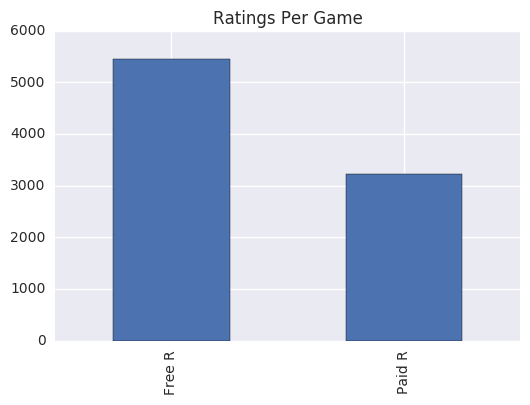
\includegraphics[width=0.45\textwidth,keepaspectratio]{freevnon-ratings-bar}
\end{figure}

\begin{figure}[H]
    \label{fig:freevnon-metacritic}
    \caption{Metacritic mean score on Free vs Non-Free games}
    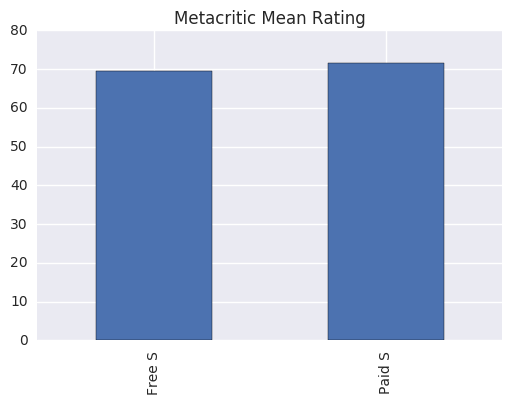
\includegraphics[width=0.45\textwidth,keepaspectratio]{freevnon-metacritic-bar}
\end{figure}


\subsection{Genre}

The most recommended genre was free to play and not action. The least
recommended genre was non-game software (see figure \ref{fig:genre-ratings}).
The highest scoring genre was sports instead of action. The lowest
scoring genre was free to play (see figure \ref{fig:genre-metacritic}).

\begin{figure}[H]
    \label{fig:genre-ratings}
    \caption{Count of recommendations from users by genre}
    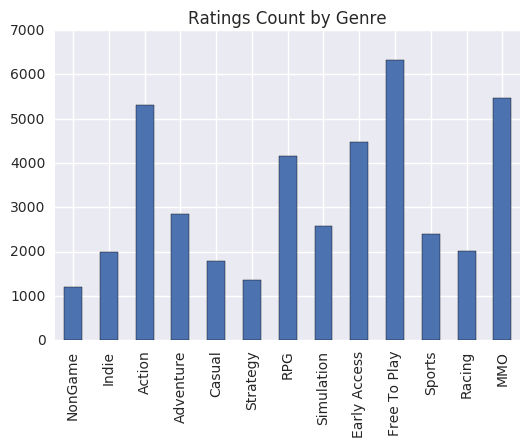
\includegraphics[width=0.45\textwidth,keepaspectratio]{genre-ratings-bar}
\end{figure}

\begin{figure}[H]
    \label{fig:genre-metacritic}
    \caption{Metacritic mean score by genre}
    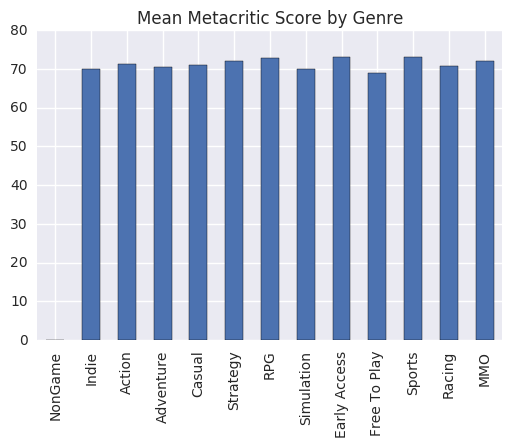
\includegraphics[width=0.45\textwidth,keepaspectratio]{genre-metacritic-bar}
\end{figure}

\subsection{Recommendations, Ratings, and Price}

Although not part of the original prediction, some relationships (or lack
thereof) were noticed. Pricing compared to Metacritic scores is mostly
uniform. The gaps for certain prices are almost entirely due to Steam's
pricing structure. Pricing compared to user recommendations is also nearly
uniform. There is a small increase in recommendations for cheaper games, but
it is not significant. Please see figures
\ref{fig:metacritic-recommendations},
\ref{fig:metacritic-price}, and
\ref{fig:price-recommendations}.

\begin{figure}[H]
    \label{fig:metacritic-recommendations}
    \caption{Relationship of Count of User Recommendations to Metacritic Score}
    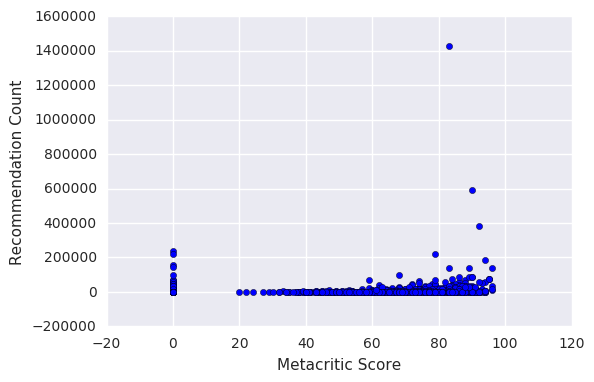
\includegraphics[width=0.45\textwidth,keepaspectratio]{metacritic-recommendations-scatter}
\end{figure}

\begin{figure}[H]
    \label{fig:metacritic-price}
    \caption{Relationship of Metacritic Score to Initial Price}
    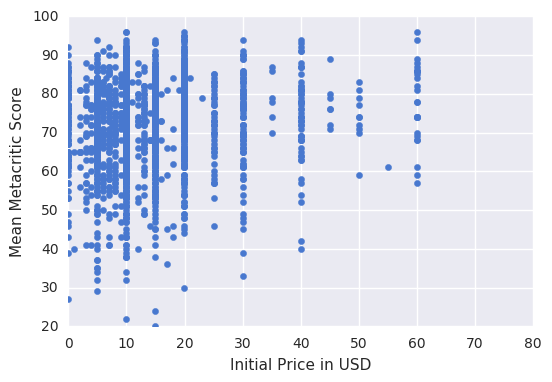
\includegraphics[width=0.45\textwidth,keepaspectratio]{price-metacritic-scatter}
\end{figure}

\begin{figure}[H]
    \label{fig:price-recommendations}
    \caption{Relationship of Initial Price to Count of User Recommendations}
    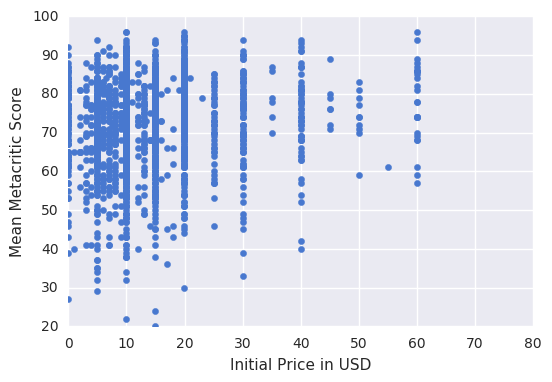
\includegraphics[width=0.45\textwidth,keepaspectratio]{price-metacritic-scatter}
\end{figure}


%%%%%%%%%%%%%%%%%%%%%%%%%%%%%%%%%%%%%%%%%%%%%%%%%%%%%%%%%%%%%%%%%%%%%%%%%%%%
%%%%%%%%%%%%%%%%%%%%%%%%%%%%%%%%%%%%%%%%%%%%%%%%%%%%%%%%%%%%%%%%%%%%%%%%%%%%

\section{Future Work}

Given a larger timespan to collect data and more sophisticated web crawlers,
more data come be pulled from Steam. This would allow for most, if not all of
the caveats mentioned before to be removed. With historical data, price
trends for games of different genres could be predicted along with the time
frames for price drops. A divided recommendation statistic could be used to
determine if certain genres get more positive reviews than others, as well as
show a correlation (or lack thereof) between Metacritic scores and positive
recommendations.

%%%%%%%%%%%%%%%%%%%%%%%%%%%%%%%%%%%%%%%%%%%%%%%%%%%%%%%%%%%%%%%%%%%%%%%%%%%%
%%%%%%%%%%%%%%%%%%%%%%%%%%%%%%%%%%%%%%%%%%%%%%%%%%%%%%%%%%%%%%%%%%%%%%%%%%%%

\section{Conclusion}

After finding a suitable platform to mine data from, the authors acquired raw
data from Steam. This data was cleaned, formatted, and processed to find
several interesting results. While all of the authors' predictions were not
proven in testing, the ones that were wrong proved to be the most surprising.

TODO: more text

%%%%%%%%%%%%%%%%%%%%%%%%%%%%%%%%%%%%%%%%%%%%%%%%%%%%%%%%%%%%%%%%%%%%%%%%%%%%%
% Bibliography
%%%%%%%%%%%%%%%%%%%%%%%%%%%%%%%%%%%%%%%%%%%%%%%%%%%%%%%%%%%%%%%%%%%%%%%%%%%%%

\nocite{*}                                 % ensure we show the entire bib
\printbibliography

%%%%%%%%%%%%%%%%%%%%%%%%%%%%%%%%%%%%%%%%%%%%%%%%%%%%%%%%%%%%%%%%%%%%%%%%%%%%
%%%%%%%%%%%%%%%%%%%%%%%%%%%%%%%%%%%%%%%%%%%%%%%%%%%%%%%%%%%%%%%%%%%%%%%%%%%%

\end{document}
